%%%%%%%%%%%%%%%%%%%%
% Thesis main file %
%%%%%%%%%%%%%%%%%%%%
%\documentclass[11pt,a4paper]{report} 										% niet recto-verso
\documentclass[11pt,a4paper,twoside,openright]{report} 		% recto-verso

\usepackage[a4paper,left=2.5cm, right=2.5cm, top=2.5cm, bottom=2.5cm]{geometry}
\usepackage[english]{babel}
\usepackage{graphicx}
\usepackage[latin1]{inputenc}		% om niet ascii karakters rechtstreeks te kunnen ingeven
%\usepackage[utf8]{inputenc}		% commentarieer deze regel uit als je utf8 encoded files gebruikt in plaats van latin1
\usepackage{natbib}
\usepackage{listings}         	% voor het weergeven van broncode
\usepackage{verbatim}						% weergeven van code, commando's, ...
\usepackage{hyperref}						% maak PDF van de thesis navigeerbaar
\usepackage{url}								% URL's invoegen in tekst met behulp van \url{http://}
\usepackage[small,bf,hang]{caption}	% om de captions wat te verbeteren
\usepackage[final]{pdfpages}		% gebruikt voor het invoegen van het artikel in pdf-formaat
\usepackage{pslatex}						% andere lettertype's dan de standaard types
\usepackage{sectsty}						% aanpassen van de fonts van sections en chapters

\allsectionsfont{\sffamily}
\chapterfont{\raggedleft\sffamily}

\usepackage{float}							% De optie H voor de plaatsing van figuren op de plaats waar je ze invoegt. bvb. \begin{figure}[H]
\usepackage{longtable}					% tabellen die over meerdere pagina's gespreid worden
%\usepackage[times]{quotchap}		% indien je fancy hoofdstuktitels wil
%\usepackage[none]{hyphenat}
%\usepackage{latexsym}
%\usepackage{amsmath}
%\usepackage{amssymb}

\usepackage{fiiw_groepT_eng}

\newcommand{\classname}[1]{\texttt{#1}}
\renewcommand{\lstlistingname}{Code snippet}

\acknowledgementspagetrue
\acknowledgements{preface}
\abstractpagetrue
\abstracts{abstract}
\listoffigurespagetrue
%\listoftablespagetrue
%\listofsymbolspagetrue
%\listofsymbols{symbols}

\opleiding{Electronics-ICT,}
\afdeling{Internet computing}

\title{Design and implementation\phantom{tj}\\
of an application for\phantom{tj}\\
controlling computer games\phantom{tj}\\
using a Kinect camera as\phantom{tj}\\
part of physical therapy\phantom{tj}}
\subtitle{ }

\forenameA{Christiaan}
\surnameA{Vanbergen}
\forenameB{Dimitri}
\surnameB{Vargemidis}
\academicyear{2016 - 2017}

\promotorA[Supervisor]{prof.\ dr.\ ir.\ L.\ Geurts}
\promotorB[Co-supervisor]{ir.\ K.\ Vanderloock}

\begin{document}
\selectlanguage{english}
\lstset{language=C++,
	basicstyle=\footnotesize,        % the size of the fonts that are used for the code
  breakatwhitespace=true,          % sets if automatic breaks should only happen at whitespace
  breaklines=true,                 % sets automatic line breaking
  captionpos=b,                    % sets the caption-position to bottom
	tabsize=2}
	
\preface

\chapter{Introduction}

There are many different reasons for requiring physical therapy. They vary from recovering from a car crash to being born with physical disabilities. The goal of these therapy sessions is respectively to make sure that the patient can recover as much as possible from his injuries or to train the muscles, preventing their situation from deteriorating.\\

Especially for children, the physical exercises performed during therapy can be demotivating. Combining these exercises with playing computer games leads to an increased willingness to continue with the exercises \cite{Brauner2013}. However, it is questionable if the classic approach related to games that incorporate physical exercises is economically sustainable \cite{Nakevska2011}.\\

The purpose of this thesis is to present a more sustainable solution to this problem in a way that offers more flexibility to the therapist, both in terms of the exercises that need to be done by the patients and the games they can play by performing the exercises.


\section{Discussion of the problem}

Patients often see exercises as a part of physical therapy as being fatiguing, monotonous and tedious. This problem is even more prominent with young patients and can quickly demotivate them, especially when the exercises are uncomfortable or painful to perform \cite{Annema2013}.\\

Computer games already exist that can support physical exercises. For instance, there are games that run on Microsoft's XBox console and accept user input through the Kinect 3D camera, or Nintendo's Wii console that use a controller with accelerometers and gyrosensors. Additionally, games exist that can run on a computer, using any combination of sensors for user input, and are specifically made for use by physical therapists and their patients. An example of such a game is \emph{Kungfu Kitchen}, which is a collection of mini-games that can be played for instance with a Kinect camera \cite{KungFuKitchen}. However, these kind of games have in common that they are very static by nature and are not often suited for the specific needs of a patient \cite{Geurts2011}. For instance, a game that focuses on arm movement is not very effective at exercising the leg muscles of a patient. In other words, concerning the therapy, this game is meaningless for a patient that had leg surgery.\\

In addition, these static games have fixed input gestures patients have to perform in order to control the action on screen. Even if the gestures perfectly fit the exercise requirements for a specific patient, the decrease in attractiveness of playing the same game over and over again is problematic and loses its long-term effect. Physical therapist Dries Lamberts has experience with children with disabilities and uses computer games as a form of exercise. The initial reaction of the children to these games is positive. They are more engaged in doing physical exercises and feel motivated while doing so. On the downside, this effect only lasts until the novelty of the game wears off. After that, the children lose interest in the game and, as such, in performing the exercises.\\

As games are expensive to develop \cite{Nakevska2011}, there is no wide variety of motion games that are tailor-made for people with specific needs and at the same time offer varied gameplay mechanics to remain interesting over longer periods of time. On the other hand, it is questionable if producing these kind of games is economically sustainable. From the therapist's point of view, the game needs to support the right type of exercises and the game itself has to be considered fun as well by the patients for them to keep invested in it. If any of these conditions are not fulfilled, therapists can be less inclined to purchase the game and patients can be less motivated to play it.\\


\section{Purpose of the research}

This thesis focuses on an application that allows for a more flexible and dynamic solution to the above discussed problem. It lets the physical therapist choose what exercises the patient has to do and how these can be used as an input to control any computer game of choice. All of this can be done without requiring the therapist to have any programming knowledge.\\

The goal is to have an application the therapist can control mainly using the Kinect camera. To provide the user with a more streamlined interaction process, switching between Kinect input and mouse input is minimized. As such, the therapist can stay in the same spot in front of the camera. Interaction needs to feel simple, efficient and natural to do. This minimizes the setup time before a patient can start playing. It is necessary to research the type of interface that is required to meet these objectives, in addition to finding out the easiest way to interact with an on-screen application using a camera for input.
\chapter{Related work}
\label{chapter: related work}

The literature study focuses on the aspects of human-computer interaction (HCI) related to gesture-based input and natural interfaces. This is followed by a closer look on research done that is directly related to using exergames as part of physical therapy.

\section{Human-computer interaction}


Gesture-based interfaces gain popularity due to the advancing technology of sensors and processors \cite{Jacob2008}. Because of this, technologies like the Kinect camera become more affordable and accessible for individuals. While interfaces supporting gesture input are referred to as natural user interfaces (NUI), this is more of a marketing term than an actual scientific designation. Natural interfaces don't feel natural to interact with just because they rely on gesture-based input. The user does not really hold the object shown on the screen to be able to interact with it naturally, so the feedback a user can get is limited \cite{Norman2010}. Direct manipulation of objects that interact with an application offer more natural feedback \cite{Shneiderman2010}. The downside is that additional objects are required for interacting with the application.\\

Notwithstanding the limited feedback when not using additional objects, gestures are powerful tools for human-computer interaction. However, gestures as an input offer a wide variety of options and with increasing popularity, a wider variation of interfaces and gestures to interact with them emerge. This is problematic as users need to get familiar with a gesture-based interface each time they encounter a new one. The full potential of this kind of interfaces can only be achieved when some kind of standard is developed and widely used \cite{Norman2010}. Frameworks based on reality-based interaction can be used to unify different research areas concerning interface design and to compare these designs to one another \cite{Jacob2008}.\\

When designing an interface and ways to interact with them, it is essential to make clear what actions are required through feedforward and what the results of those actions are through feedback. Because of that, feedback and feedforward are powerful tools. Designing a gesture-based interface comes down to trying to have natural coupling between action and reaction. Natural coupling can be evaluated by six aspects: time, location, direction, dynamics, modality and expression \cite{Wensveen2004}. The time aspect requires that there is no perceivable delay between the execution of an action and the result shown on the screen. The direction and location of action and reaction have to match as well. The modality is tightly coupled to the dynamics and direction, as it must be possible to visually perceive the result of an action. Modality however is not limited to visual cues. Auditive feedback on certain actions can improve the coupling between action and reaction as well. Visual representations of the reaction must be similar to the action in terms of dynamics, meaning that the speed and acceleration of both have to match. The aspect of expression is also related to the dynamics of the action. This means that the interface has to visually represent the way the user performed an action. If the action is done quickly and not very accurately, it must be reflected by the interface. If feedback as well as feedforward are able to support these six aspects, the user perceives the interface as more intuitive to interact with and action and function become more closely related. The more aspects are fulfilled, the higher the natural coupling is. \cite{Wensveen2004}\\


\section{Exergames as part of physical therapy}

Using games as part of physical therapy has been the subject of many research papers \cite{Geurts2011}\cite{Hondori2014}\cite{Lange2012}\cite{Chang2011}. An example of an exergame is Kungfu Kitchen \cite{KungFuKitchen}. Since it is found that exergames improve motivation \cite{Brauner2013} and offer physical, social and cognitive benefits, they are more frequently used by physical therapists \cite{Peng2011}\cite{Staiano2011}.\\

While the reliance of the patient on the therapist can be reduced by using exergames, the rate of rehabilitation does not increase \cite{Dahl2014}. Because of a decreased reliance on the therapist, he can focus on supporting the patient during play \cite{Annema2013}. Since these games can be a tool of aid to the therapists, it should not hinder them in any way, nor increase the amount of work or effort they put into the preparation of a therapeutic session. For this reason, setting up everything needed before starting to play should not take up too much time. This includes but is not limited to: the time to set up the used sensors, the time the application takes to start up and the time needed for the application to process data.\\

Within the same mindset of making life easier for physical therapists, the application can be a useful source of information for the therapist, as it can provide him with details of the progress his patient is making either during one session or over the course of long-term therapy. Again, this allows the therapist to focus on the essence of the therapy instead of on taking notes, keeping close track of how the patient is doing \cite{Annema2013}.\\
\chapter{Design}

The focus of the application is to simplify the setup process for the therapist, ensuring that he does not require programming experience or knowledge about the underlying system, while still providing all tools needed for the patients to play a game using gesture input.\\

The developed application can roughly be split up into three major parts. Firstly, the graphical user interface (GUI) allows the therapist to interact with the application, providing him with feedback and feedforward on inputting exercises for the patients. Secondly, gesture recognition is done as part of machine learning using support vector machines (SVM). Thirdly, all other back-end software connects the first two parts and provides a structure in which all data is managed and stored.


\section{Description of the application}

The application uses Microsoft's Kinect 2.0 camera as an input device. The principle is that games can be played by first recording gestures and then performing them. In order to set up the application, there are a number of steps to be taken and guidelines to keep in mind.


\subsection{Principle}

When playing a computer game the conventional way, a person can interact with the game by pressing a keyboard key. Pressing the key then results in an action on the screen (see figure \ref{fig: overview_basic_interaction}).\\

\begin{figure}[H]
\begin{center}

\includegraphics[width=6cm]{KUL.png} %THIS IMAGE IS A PLACEHOLDER
\caption{\emph{Overview of the interaction between a person and a computer game under conventional use}}
\label{fig: overview_basic_interaction}
\end{center}
\end{figure}

The developed application can be seen as an additional element between a person and pressing a keyboard key for controlling a game. In short, the application allows a person to remotely press a key by performing an exercise chosen by the physical therapist (see figure \ref{fig: overview_application_interaction}).\\

\begin{figure}[H]
\begin{center}

\includegraphics[width=6cm]{KUL.png} %THIS IMAGE IS A PLACEHOLDER
\caption{\emph{Overview of interaction between a person and a computer game using the developed application}}
\label{fig: overview_application_interaction}
\end{center}
\end{figure}

More in detail, the physical therapist comes up with exercises that fit the needs of a patient. He uses the Kinect camera to interact with the application via a GUI. Next, the therapist lets the application record what exercises need to be done by the patient. Using all of the recorded exercises, an SVM model is created, which is used to predict what exercise is performed by the patient while playing a game.\\

The therapist assigns a keyboard button to each of the exercises. This means that when the patient mimics one of the therapist's exercises, a keyboard button is pressed. To start playing a game, the therapist can choose any game or let the patient choose his preferred game. This can be any type of computer game and includes, but is not limited to: browser games, games that need to be downloaded and installed, pre-installed games that come with the operating system,\ldots If this application is running in the background while a computer game is opened, performing an exercise indirectly presses the button that is linked to the exercise. By doing this, the patient can interact with the game.\\

By mapping exercises to keyboard buttons, a vast amount of existing games can be played using gesture-based input. It is however limited to button presses. Pointing with the cursor like when using a mouse is not supported by the application. The reason is that every gesture performed is seen as one single action. The gesture of pointing to a specific spot on the screen could overlap with one of the exercises the therapist wants to use. This results in undesirable behavior and negatively impact the gaming experience for the patient. A way to solve this problem is to predefine a specific gesture that activates the \emph{pointing mode}. In this mode, it is only possible to point to something on the screen or switch back to the \emph{gesture mode}. However, this gives more responsibility to the therapist, who has to remember what that specific mode changing gesture is and that he cannot input that gesture as an exercise for the patient. In addition, defining a preset gesture means that not every patient has the ability to perform it, as some may not be able to move an arm or a leg, for instance. Since, from an end-user point-of-view, this setup is confusing and undoes the application's elegance of simplicity, only games can be played that require only button presses as an input.\\


\subsection{Setup}

Before the application can be used, the user has to download and install the necessary drivers in order to use the Kinect 2.0 camera. This is only required once per device it is used on. To connect the Kinect 2.0 camera to a computer, an additional adapter is needed so it can be connected using a USB 3.0 port (see figure \ref{fig: kinect}). The use of the Kinect camera requires a socket.\\

\begin{figure}[H]
\begin{center}
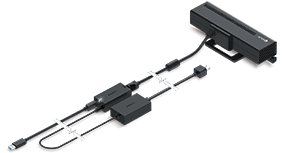
\includegraphics[width=8cm]{KinectAdapter.png}
\caption{\emph{The Kinect 2.0 camera connected to the adapter}}
\label{fig: kinect}
\end{center}
\end{figure}

The camera has to be placed horizontally in order to function correctly. The distance between the user and the camera may vary between 1.5 and 4 meters, depending on the height of the user and the size of the used screen (see figure \ref{fig: kinect_setup}). The camera can be tilted upwards or downwards. The chosen angle depends on the height of the camera. Both can be chosen freely by the user, but the user has to ensure that he is fully visible at the position he stands. The GUI allows him to verify this. A possible configuration that works well is to have to Kinect camera pointing straight ahead on a table with a height of approximately 0.8 meters.\\

\begin{figure}[H]
\begin{center}

\includegraphics[width=8cm]{KUL.png}
\caption{\emph{Setup for the Kinect camera}}
\label{fig: kinect_setup}
\end{center}
\end{figure}

Before starting the application, it is recommended to put the executable file in a directory that does not need to change of the course of multiple uses. The reason is that a subdirectory is created in the same directory, containing all data files of saved exercises. As long as this data folder and the executable are in the same directory, all previously recorded exercises are loaded when starting the application. If they get separated, the application still can be used, but it appears as if there are no saved exercises and it creates a new data folder in the directory the executable is stored.\\


\section{Graphical user interface}

%DELETE THE ITEMIZATION BELOW
\begin{itemize}
\item Procesbeschrijving, opties tussen verschillende types van interfaces (mime/music conductor)
\item Experimentele manier om tot prototype te komen door gesprek met kinesist
\item Beschrijving van de voorgestelde oplossing, beelden van de GUI, bespreking
\item Klassendiagramma voor GUI
\item \ldots
\end{itemize}

A large part of this thesis was focused on the design and implementation of a user-friendly interface that can be controlled via input from the kinect 3D camera. The reasoning behind this is that the user does not want to run back and forth from the standing position in front of the kinect and the keyboard. Many interfaces have been design for use with the kinect but they are generally only used to get the game and are therefore made up of simple button and scrollbars to select your option. In this section the process of developing the user-interface and the eventual implementation is discussed.

\subsection{Prototypes}

The goal with this part of the thesis was to find a new way of interacting with a user-interface using the kinect 3D-camera that feels natural to the average user, this despite  \textbf{NORMAN's} claims that the  term natural user-interfaces, that is often used to describe interfaces controlled with 3D-cameras, are not natural because  of \textbf{REASONS}. This means that we will try to avoid using standard WIMP (Window, icon, menu, pointer) elements such as pushbuttons and scrollbars. A brainstorm session with the eventual user, the physical therapist, would give us fresh idea's on how the user will expect to interact with a user interface using his body or sound. The expectation was that 2 distinct observation would be made: how the user would wish to interact with the user-interface and how they would expect the flow of the program. 

 {\large COMMENT: is WIMP de juiste term in het vorige stuk? }
 {\large COMMENT: hadden wij toen al dat visuele stappen plan? ik denk het niet he }

In our process during this session the idea was to keep the user from being influenced by our idea's or by obvious solutions.To start we would only explain the basic concept of our application and the abilities of the kinect 3D-camera. Then the subject was asked how he would imagine every expect of the application, a few questions from the script were: what information would you expect to see on the screen, how would you start a recording, what would you want to see during recording, etc. 

To find out whether such a brainstorm session would yield any viable results brainstorm sessions with our relatives were conducted first. An important remark to make here is that we tried to do this with people who are not from any software related area's so they had little foreknowledge about how user-interfaces are designed apart from their own experience with using programs. The 2 iterations were performed with four subjects, the first test was with two males and the second was with two females, of both genders there was one person around 25 years old and one around 55 years old. Each subject was interviewed completely separate to minimize the influence they had on each others ideas.

The sessions were very taxing for the test subjects, the concept we tried to introduce was too abstract and foreign to them. This causes them to be shy with proposals, even after being ensured that there are no bad ideas. It seemed to give them the feeling that they are be not smart enough to make good proposals. As a result they fell back on proposing  familiar UI elements or concepts such as pushbuttons or voice-control. Getting locked into a mindset that we were designing games to play with the kinect was also a minor issue, thereby answering the questions with that in mind, which was not the point. After 2 iterations with minor changes between them, we decided not to subject the physical therapist to this kind of questioning. Setting up a meeting would waste to much of his precious time with little gain to us. Worse, it might instill the physical therapist with a feeling of dread for our next meeting which might reduce his level of co-operation. 

 {\large COMMENT: hier mag we een of andere splitsing komen die duidelijk een onderscheid maakt tussen dees 2 delen}

Instead we decided to brainstorm with each other and our supervisor Prof. Geurts to develop a few paper prototypes that we can eventually show to the physical therapist to see which one seems the most user-friendly. The two mayor interaction patterns that came out of this brainstorm session we call hints and mime. In the rest of this chapter the abbreviation UI is used to say user interface and a UI element is a button, scrollbar or any other element that the user can interact with. When discussing the different concepts we often refer to a movement by the user or position that is taken that activates a function in the program as a sign.

The hints pattern implies that the screen is largely devoid of UI elements and actions are performed when the user does a certain movement or takes a certain position, for example, the user forms an cross with his arms to delete a recording.  The lack of feed forward that this implies means the user should learn all of the signs at the start of application, putting a large strain on the user's cognitive ability which is not ideal. Alternatively, all possible action could be displayed on the screen around the user with a depiction of the sign. Though this would put less strain on the user's cognitive abilities, he would still have to focus on these pictures and try to figure out what sign they depict. But what if the sign is a movement? It is impossible to depict is statically so how can you make this clear without distracting the user with constant moving pictures. A more significant problem might be the fact that position and movements might be recognized by accident, an undo movement could partly solve this but you also need a redo button to compensate for any accidental undo-activations.{\large COMMENT: iets over het perongeluk activeren bij on aandachtig zijn.}  The only real benefits to using the hints pattern is that activating an action can be done from anywhere and it could be faster once the user has mastered the signs, though this depends on the ease of performing the signs and the delay between a sign and the corresponding action in the program.\\
{\large COMMENT: make the signs so that the link between the sign and the action is similar to the meaning it has in everyday life, culture dependency .}\\

The mime pattern, as the name suggests, is the act of mimicking an action that is needed to act on everyday objects such as opening a door. But where an mime artist does this without any indication of that object being there, here an image of ,for example, the door would be displayed on the screen. The technical term for such a UI element is a metaphor because the function is similar to what a user would do with the object in real life. The power of this pattern is that the user should immediately recognize the UI element, know how to interact with it. To achieve the best effect, the UI elements that are chosen should need signs that the user has done frequently already, so that doing them feel natural and familiar. An extra user friendly characteristic would be if the sign performs a function that is similar the real life such as going to a different screen when opening the door. \textbf{Wensveen} already said that for this to work correctly feedback is crucial, the reaction of the UI element must match the expectations of the user otherwise he will be confused and the flow of the program is interrupted. Disadvantages is that you cannot activate every action from anywhere and it might be slower because of that.  \\
{\large COMMENT: Allows the use of affordances }  \\
{\large COMMENT: look in notes HCI for extra idea's from the literate study }\\


Our opinion is \textbf{(and that of other?)} is that one should not mix the 2 patterns because the user will expect to interact with everything on the screen when using the mime pattern if one action is activated using the hints pattern the user will forget and be confused if there is no indication of this and if there is indication the user will likely try to interact with the indicator of the sign as a button which will not have the desired effect. Combination with regular WIMP UI elements, such as pushbutton or scrollbars, is possible\textbf{(is it possible?)} for both patterns but it combines better with the mime pattern because it requires the user to point at a specific area in the UI which would detract from the idea of being able to do every action everywhere in the hints pattern. To sum up in the mime pattern the behavior of the UI elements are simple and obvious but possibly more inefficient, like pulling a handle on a slot machine to spin the slots. While the hints pattern is more abstract and complex, but should allow a more efficient interaction once mastered.

With these patterns in mind the design of the paper prototypes focuses more on designing UI elements and methods with which the user can interact that is simple, fast, ergonomically, feels natural and is not taxing to the user physically and cognitively while being practical and not easy to activate accidentally. The regular way of testing paper prototypes is by presenting the user with a paper version of the UI (hence the name) and whenever the user touches a UI element the designer manually changes the paper prototype to reflect the activated action. This kind of testing absolutely not suited for this kind of designing, it is more to assess the placement and shape of UI elements and the general flow of a program. What was needed here is a way to interact with the paper prototypes in a way similar to how the real program would work but without having to code the whole program. For that reason we took 2 example programs from Microsoft's kinect SDK and made some adjustment to show the user in front of the paper prototype, these applications will be discussed further down this chapter. \\
{\large COMMENT: out of idea's to be continued }\\
 
 Regarding how the user is shown on the screen there are four viable options : \\
 1. A real image of the person as the camera films it is shown.  \textbf{reference to fig 1? A} \\
 2. A semi-transparent schadow of the user is shown. \textbf{reference to fig 1? B} \\
 3. A puppet that copies the user's movement is shown.  \textbf{reference to fig 1? C} \\
 4. No body is shown, only images that portray the position and state of the hands are shown\textbf{reference to fig 1? D}\\ \\
 
 \begin{figure}[H]
 	\begin{center}
 		
\includegraphics[width=7cm, height=7cm]{KUL.png}
 		
\includegraphics[width=7cm, height=7cm]{KUL.png}
 		
\includegraphics[width=7cm, height=7cm]{KUL.png}
 		
\includegraphics[width=7cm, height=7cm]{KUL.png}
 		\caption{\emph{types of visualizations of the user}}
 		\label{fig: a: the UI with real image of user, b: the UI with semi-transparent shadow, c: the UI with puppet, d: the UI with only hands }
 	\end{center}
 \end{figure}
 
 
 A real image of the person is the most identifiable for the user because it is literally an image of himself but this doesn't mean that it would be the best option to use in interacting with the UI. Though it has the advantage that it is crystal clear with movement the user caried out which is good for recording and replaying exercice. The most important issue is that the image is taken from the front so the image of the screen is facing away, so unless the UI elements are drawn on top of the user's image it is hard to imagine you are grabbing a handle or pushing a button on the UI. Placing the kinect camera behind the user to solve this problem, is technically not possible because an important part of the kinects person recognition is based on recognition of the the facial features. This would also require a very large amount of room to operate because you need to have a distance of atleast a one meter from the screen in front of the user and at least 1.5 m from the kinect at the back. When the UI elements are drawn behind the user, he will also obscure any elements directly behind him. Another issue is that most people are not comfortable with an image of themselves being displayed on the screen which could detract from the user experience. The physical therapist we interviewed, who works in a school for disabled children, also noted that this might cause legal problems with parent who do not want unauthorized footage of their child being stored. A final technical issue is that displaying the real image of the user is very resource intensive and in our case it would sometimes cause the program to lag. \\
 {\large COMMENT: Why can't the real image also be transparent?}
 
 A semi-transparent shadow would solve the legal issue, the discomfort experienced by users and it also solves the problem of the image facing away from the UI because there are almost no features that indicate which way the image is facing, making it look like the shadow is facing towards the UI. By making the image semi-transparent any UI element behind the user can still be seen. A disadvantage is that it is harder to identify subtle differences between similar recordings. It is also still very resource intensive, trying to optimize this was beyond the scope of this thesis.
 
 
 A puppet that copies the movements of the user has similar benefits to the shadow and can be transparent or non-transparent. It is far less resource intensive but makes it even harder to distinguish similar recordings from each other.
 
 Showing no body and only hands can obviously only be used to interact with the UI and not for the recording of an exercise. It removes all distractions from the screen and shows only the states that are essential to the user to interact with the UI. But because of this the interaction might feel less natural to the user.
 
In total 6 paper prototypes are created ranging from obvious prototypes using mostly mime pattern elements and metaphors to more abstract prototypes where more elements of the hints pattern and standard WIMP concepts are used with less mime pattern elements. 
The first four paper prototypes are only the screen in which the user can record one exercise multiple times to provide the data for the SVM as discussed in \textbf{REFERENCE TO CHAPTER?}. They use a schadow image of the user to control the UI. The other two prototypes are menu's to browser to a recording and replay it while the user only sees his images of his hands. This list sums up all the prototypes: \\

1. A UI with mostly mime pattern elements and metaphors. \\
2. A UI that combines mime patterns with standard WIMP elements. \\
3. A UI that also combines mime patterns but with more WIMP elements. \\
4. An alternative mime pattern element for the scrollbar only. \\
5. A UI that combines the hints pattern with WIMP elements. \\
6. A UI that combines the hints pattern with more WIMP elements.\\ \\

In this thesis only three of these prototypes are discussed to show the kind of elements that were experimented with, these are: the first prototype, the third and the last, a more detailed description of the rest of the prototypes can be found in \textbf{appendix A}.\\

{\large COMMENT: should I talk about some general rules we kept to? like don't place buttons too low}

The first paper prototype, that can be seen in \textbf{ fig:2}, mostly uses the mime pattern and metaphors, the orange color is used to indicate a possibility for an action. On the right the door on the side says exit and would swing open when the user grabs the orange handle an pulls to the left. On the top of the screen a collection of recordings can be seen pinned to a scrollbar with orange thumbnails, the arrows on the sides imply that the recordings can be moved. The user would grab the orange indicator bar to browse the recordings. To delete a recording the user grab the thumbnail of that specific recording and drag it to the recycle bin to release it there. The user can display the recording by dragging it to the projector on the left side of the screen with would display the recording on the screen where the big 1 is displayed. In the middle a camera with his lens pointed towards the user is displayed, by moving his hand forward on the "opnemen" button the user could start a recording.

\begin{figure}[H]
	\begin{center}
		
\includegraphics[width=16cm, height=9cm]{KUL.png}
		\caption{\emph{The first paper prototype}}
		\label{The first paper prototype}
	\end{center}
\end{figure}

{\large COMMENT: START MOVE TO APPENDIX}

The second paper prototype combines mime pattern elements with more standard WIMP elements to streamline the process. In \textbf{ fig 3} the first screen can be seen. On the left of the screen the screen can be exited by grabbing the orange part of the lever and pulling it downwards. A new recording can be started by grabbing the orange part of the cord and pulling downwards. The record screen as seen in \textbf{ fig 4} is now shown. The window shown is what is going to be recorded, the red one shows where the program will count down from 3 until the recording starts allowing the user for some time to get to his start position. All other UI elements are grayed out to indicate that they are not available to interact with. Once the recording is finished the program returns to the screen in \textbf{ fig 3}. When the user moves into the orange circle on the ground the program switches to a different mode as seen in \textbf{ fig 4} which is called the manage screen. The window on the right of the screen will replay the recording that is highlighted in orange in the scrollbar automatically. The user can pause this function by pushing the orange slide button above the scrollbar to the left, grabbing it is not necessary. Each block in the scrollbar is linked to a recording and contains a static previews of their recording. The recording that is highlighted orange can be pushed into the trash, grabbing it is also not necessary here. On the right side of the user is an orange scroll wheel that is connected to the scrollbar to indicate it's association with the scrollbar, the orange tint difference can be used to indicate the speed and the direction in which the wheel is turning. The idea is that the user can move an right hand over the scroll wheel to scroll through the items in the scrollbar, simultaneously the user can use his left hand to delete an item in the scrollbar. The gray block next to the scrollbar is an indication of position within the scrollbar.

\begin{figure}[H]
	\begin{center}
		
\includegraphics[width=16cm, height=9cm]{KUL.png}
		\caption{\emph{The standard screen of the second paper prototype}}
		\label{The standard screen of the second paper prototype}
	\end{center}
\end{figure}

\begin{figure}[H]
	\begin{center}
		
\includegraphics[width=16cm, height=9cm]{KUL.png}
		\caption{\emph{The record screen of the second paper prototype}}
		\label{The first paper prototype}
	\end{center}
\end{figure}

\begin{figure}[H]
	\begin{center}
		
\includegraphics[width=16cm, height=9cm]{KUL.png}
		\caption{\emph{The manage screen of the second paper prototype}}
		\label{The first paper prototype}
	\end{center}
\end{figure}

{\large COMMENT: END MOVE TO APPENDIX}

The third paper prototype in the list combines mime pattern elements with more standard WIMP elements to streamline the process, it can be seen in \textbf{ fig 3}. On the right of the screen is a lever that is activated by grabbing the orange part of the lever and pulling it downwards causing the user the leave this screen. The record button is a pushbutton that the user activates by moving his hand forward over it. This action activates the record screen as seen in \textbf{ fig 4}. The window shown is what is going to be recorded, the red one shows where the program will count down from 3 until the recording starts allowing the user for some time to get to his start position. All other UI elements are grayed out to indicate that they are not available to interact with. Once the recording is finished the program returns to the screen in \textbf{ fig 3}. When this is activated the screen changes to  On the left is a scrollbar that contains elements that represent previous recordings. These show a static representation of their recording. On the right of it there is a scroll wheel in orange with which the user can scroll through the scrollbar by simply hover his hand above it. When the user stops scrolling the elements are locked into a position as is it is shown in \textbf{ fig 3}. By hovering over it the user can slide the top element into the "THRASH" or "PLAY" area to play or delete the element. 

{\large COMMENT: Is this really necessary in such detail?}

\begin{figure}[H]
	\begin{center}
		
\includegraphics[width=16cm, height=9cm]{KUL.png}
		\caption{\emph{The standard screen of the third paper prototype}}
		\label{The standard screen of the third paper prototype}
	\end{center}
\end{figure}

\begin{figure}[H]
	\begin{center}
		
\includegraphics[width=16cm, height=9cm]{KUL.png}
		\caption{\emph{The record screen of the third paper prototype}}
		\label{The record screen of the third paper prototype}
	\end{center}
\end{figure}

The last paper prototype is a combination of the hints pattern where the user has to close his hand over the element with which he wants to interact to open een typical WIMP element called a context menu with which the user can interact. The user can only see images of his hands as discussed earlier in this chapter. It start af with a small tutorial screen as seen in \textbf{ fig 4}, when the user closes his hand the context menu as seen in \textbf{ fig 5} when the user slides his closed fist towards any of the elements it reacts as seen in \textbf{ fig 6} to indicate the the option is chosen. Throughout the prototype the user can interact with the chosen recording as seen in \textbf{ fig 7}, in this instance he can choose between playing the recording, deleting it or canceling the current menu.

\begin{figure}[H]
	\begin{center}
		
\includegraphics[width=16cm, height=9cm]{KUL.png}
		\caption{\emph{The first tutorial screen of the last paper prototype}}
		\label{The first tutorial screen of the last paper prototype}
	\end{center}
\end{figure}

\begin{figure}[H]
	\begin{center}
		
\includegraphics[width=16cm, height=9cm]{KUL.png}
		\caption{\emph{The second tutorial screen of the last paper prototype}}
		\label{The second tutorial screen of the last paper prototype}
	\end{center}
\end{figure}

\begin{figure}[H]
	\begin{center}
		
\includegraphics[width=16cm, height=9cm]{KUL.png}
		\caption{\emph{The third tutorial screen of the last paper prototype}}
		\label{The third tutorial screen of the last paper prototype}
	\end{center}
\end{figure}

\begin{figure}[H]
	\begin{center}
		
\includegraphics[width=16cm, height=9cm]{KUL.png}
		\caption{\emph{An example of how the user would interact with and element of the last paper prototype}}
		\label{An example of how the user would interact with and element of the last paper prototype}
	\end{center}
\end{figure}

{\large COMMENT:THE PAPERPROTOTYPE USERTEST}

The mayor goal of this user test is to see how the user interacts with the different paper prototypes, how fast can he do the required actions, what he thinks of the signs whether they feel natural or not and which one of the paper prototypes speak to him the most. 

The kinect is placed on a table of regular height and the user is asked to stay within 2 to 4 meters distance from the camera. The screen with the UI is placed directly behind the kinect camera.

The user is first introduced to the concept and flow of our program through the use of a simple schematic with the required steps of the program as seen in \textbf{ fig 5}, to bring the user up to speed with what is necessary to operate the eventual progam. {\large COMMENT: WHERE TO INTRODUCE THIS?} Then a small demo program, to show the capabilities of the concept and the kinect is shown, to give him an idea of the possibilities and the end goal of the program. After some more introductory questions the user is assured that he is never at fault and that we are responsible for any misunderstandings he might have. Before the actual tests permission is asked to film the proceedings of the tests. During the test we also remind him that we like the hear his thoughts on what he sees and thinks.\\

Then the user is asked to interact with the prototypes using the kinect. To mimic the functionalities of the screen a Wizard of Oz method is used to change the screens whenever the user performs the required action. Some prototypes still require some explanation but generally the user is only assisted when he is completely stuck and at the end of every prototype an explanation of the intend is given. At the end we go through every prototype again without the kinect to reflect about the performance of every prototype. The user is asked to select a personal favorite.

In total four candidates were subjected to this user test of which were one physical therapist and three relatives or friends but this paragraph will focus on the results with the physical therapist supplemented with the results of the others, thereby the physical therapist is refered to as "the user" and the others as "the other users". It is important to mention that the user has previous experience with kinect games which sometimes influenced his reaction, such as he did not know that he could move his hand forward to mimic pushing a button. For the first prototype  \textbf{ fig 2} The user was trying to interact with UI elements that were not intended to be interacted with, he later indicated that he did not see the metaphors as they were intended and that the screen was to hectic. After the explanation of the first prototype the user commented that he now understood it the goal of the screen much better. Most of the other users also made the same remarks about the first prototype. The rope UI element such as seen in the second prototype in the \textbf{ appendix} was clear to him how to interact with it but he had no idea how to interact with the scroll wheel to scroll through the scrollbar. The lever to leave the screen was clear but he did not like the Others users indicated that they expected the UI to react as if it were a touchscreen. 
{\large COMMENT:TO BE CONTINUED}








%TODO alles over de prototypes (ook experimentele strategie uitleggen)

\subsection{Description of the interface}

The end design looks as seen in \textbf{ fig simple picture} From left to right the user can see a gray box in which a recording can be replayed, this is a typical WIMP element becuase it does not have any elements to it that can be seen as a metaphor to anything the user is familiar.Right of this there is the rope as seen in prototype 2 which is a very distinct mime pattern element and a simplified version of the scollbar containing the recordings with the currently selected recording highlighted in orange. The user can slide this element to the "DEL" bar to delete the element. The black bordered box at the feet of the puppet represent the ground on which the puppet walks on so it does not appear to float in mid air.

Though we had previously established that the schadow was the most naturel way of representing a user in the interface. Performance issues forced us to resort to using the puppet image. The reason why the puppet is not semi-transparent is because the joints are more visible because two semi-transparent images are drawn on top of each other which combine into a less transparent color. This breaks the unison of the puppet's coloring making it seem less human which would be a distraction that detracts from the experience of the user. Another detail of the puppet is that the centerpoint of the spine is fixed in the vertical direction but not in the horizontal direction. This eliminates any dependency on the position of the camera so that, as long as the body is in the field of vision of the kinect, the user can always reach every UI element on the screen. This measure introduces two different problems: the biggest problem is that when the user tries to squat the puppet will lift its feet instead of lowering his torso, this might cause confusion and does not feel natural. The other problem is that the user cannot reach any UI element that is placed where the it could only be reach by bending downwards. This is not seen as a big problem because such a movement is very taxing for an adult to perform. The puppet is free to move in the horizontal direction but there is an offset on where the puppet is drawn so that the puppet appears to stand between rope and the scrollbar drawn more toward the right of the screen when the user is standing right in front of the kinect, normally the screen will also stand behind the kinect so that the user can look straight forward when interacting with the UI. The depth coordinate in 3D space is also set to a fixed distance before conversion to a 2D screen to ensure that the puppet is always drawn to the same size no matter how far the user is standing within the vision field ofcourse.

\begin{figure}[H]
	\begin{center}
		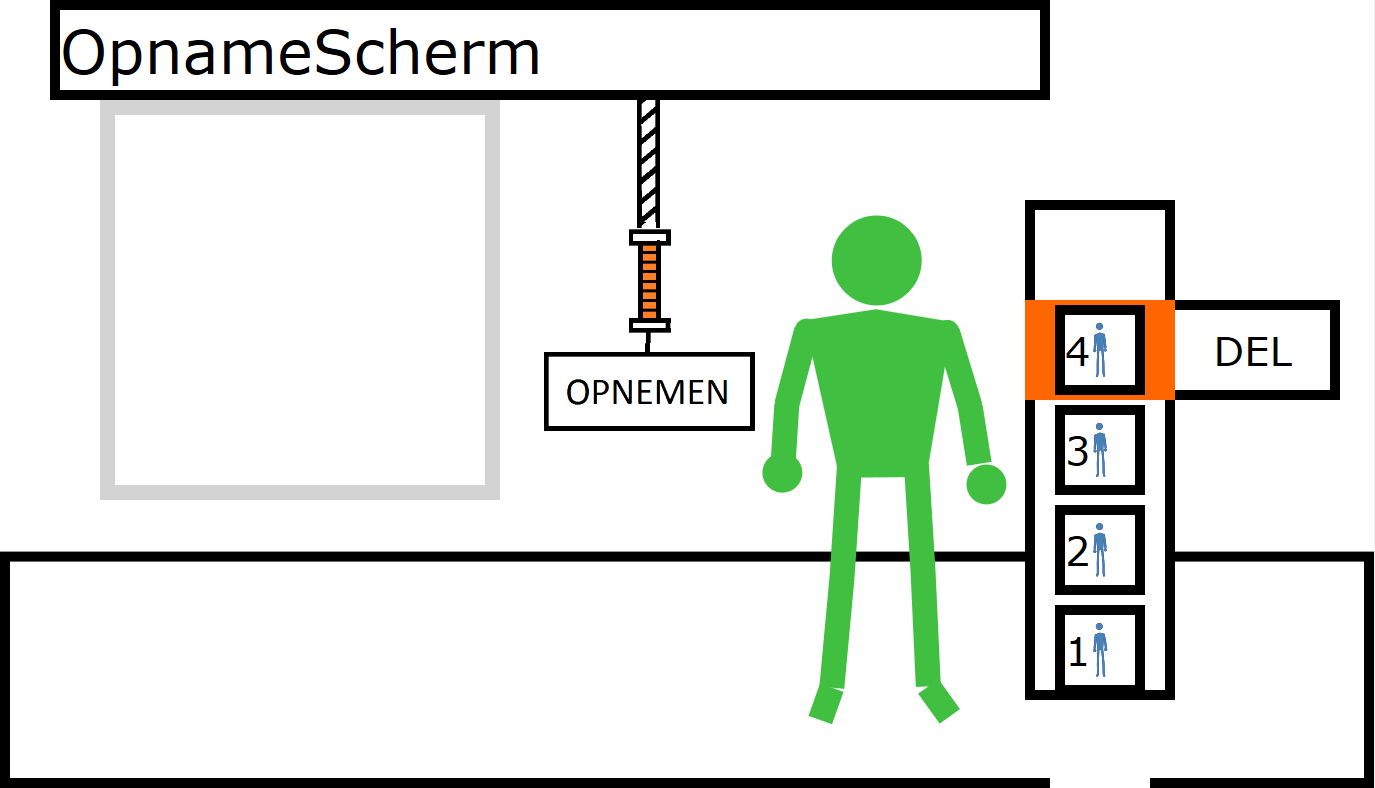
\includegraphics[width=16cm, height=9cm]{figures/1_screen_with_user.png}
		\caption{\emph{The regular view of the end design of the UI}}
		\label{The regular view of the end desing of the UI}
	\end{center}
\end{figure}


An important aspect of the UI is the color coding that is consistent throughout the UI except on the puppet itself though it should be apparent that the puppet is not much more than a representation of the user. {\large COMMENT: the puppet doesn't activate anything without interaction with any of the UI element to keep in line with the general pattern of the UI} This should give the user extra feedforward about what the consequence of their action will be. Orange is indication of interaction possibilities, green means a hand is hovering over the element, blue gives information about what happened or will happen after an action and red indicates a more serious action is about to be activated. The exact meaning of all these color codes will become clear during the description of the UI.

Since it is important for the user to know when the system sees that it is grabbing the rope, the UI provides feedback to the user by coloring the hands green when they are open and red when the user makes a fist.

When the user hovers his hand over the orange handle of the rope the handle turns green indicating that it can now be grabbed. When the user closes his hand then the handle turns red to show the user that he is pulling it. The dynamics for pulling the rope are simple, between the starting position and the end position, which is below the starting point, the rope will make the same relative movement in the vertical direction as the user does with the center of his hand. In this way the interaction is linked in time, speed, direction, dynamics and location user's hand {\large COMMENT: FRAMEWORK REF?}. When the rope is near to his end position the record screen is activated. There is no progression bar to indicate how far the user is from activating the function because generally the action of pulling a rope is very sudden and fast, as long as the function is activated before the user runs out of momentum this kind of feedback is not needed here. In the normal state the handle guards are not colored because the indication of the action area is clear enough and a person would not normally grab a handle by the handle guards, they are however colored green and red to make it more apparent to the user that they are acting on it. 

\begin{figure}[H]
	\begin{center}
		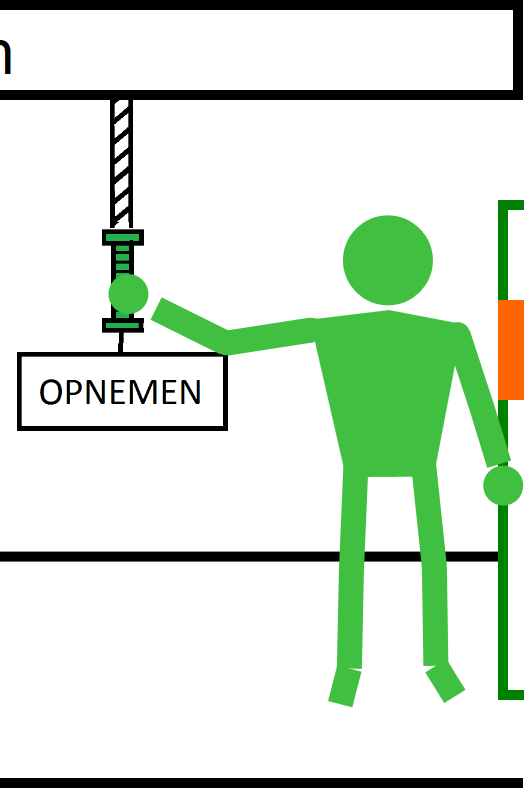
\includegraphics[width=6cm, height=8cm]{figures/2_hover_over_rope.png}
		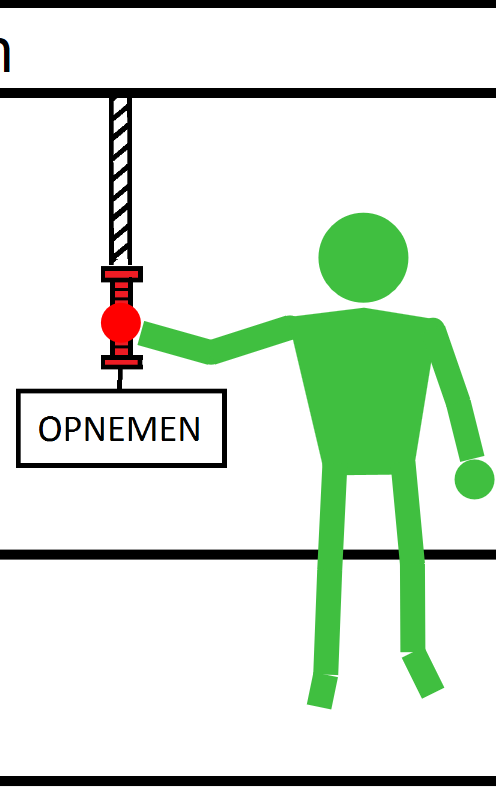
\includegraphics[width=6cm, height=8cm]{figures/3_grab_rope.png}
		\caption{\emph{Reaction of the rope handle: a) when hovered over, b) when grabbed}}
		\label{The regular view of the end desing of the UI}
	\end{center}
\end{figure}

The rope activates the screen seen in \textbf{ fig 8}. In this screen a seperate window is openend with a a scaled version of the puppet, another typical WIMP element. The large change in the UI clearly indicates that the user is in a different mode. Here the puppet is also fixed in the X direction to indicate correctly how the program will see the exercice. To avoid confusion the window is opened on top of the last position in which the user was before pulling the rope. Since the goal of this screen is to record one exercice multiple times two static puppets are drawn behind the user, the light blue puppet shows the starting position and the dark blue puppet shows the end position of the movement. Care has been taken to choose a color that does not conflict with the green of the user's puppet and doesn't overpower it by being to bright while still being clearly visible and distinguishable. The color also follows the color code defined earlier in this chapter since it gives information about the first recording. The message "Get Ready" is shown for 1 second before changing to a count down of 3,2,1,Go!. At "Go!" the window's edges turn red to clearly indicate that the program has started recording the user's movements. An example of how this would look can be seen in \textbf{ fig 9}. The program stops recording when the user remains still for certain amount of time. After that the text changes to "Done!" and after 0.5 seconds the screen return to \textbf{ fig 8}. The result is that a new element in the scrollbar is added to the top. It is given the next number and set into the orange selection area.\\



\begin{figure}[H]
	\begin{center}
		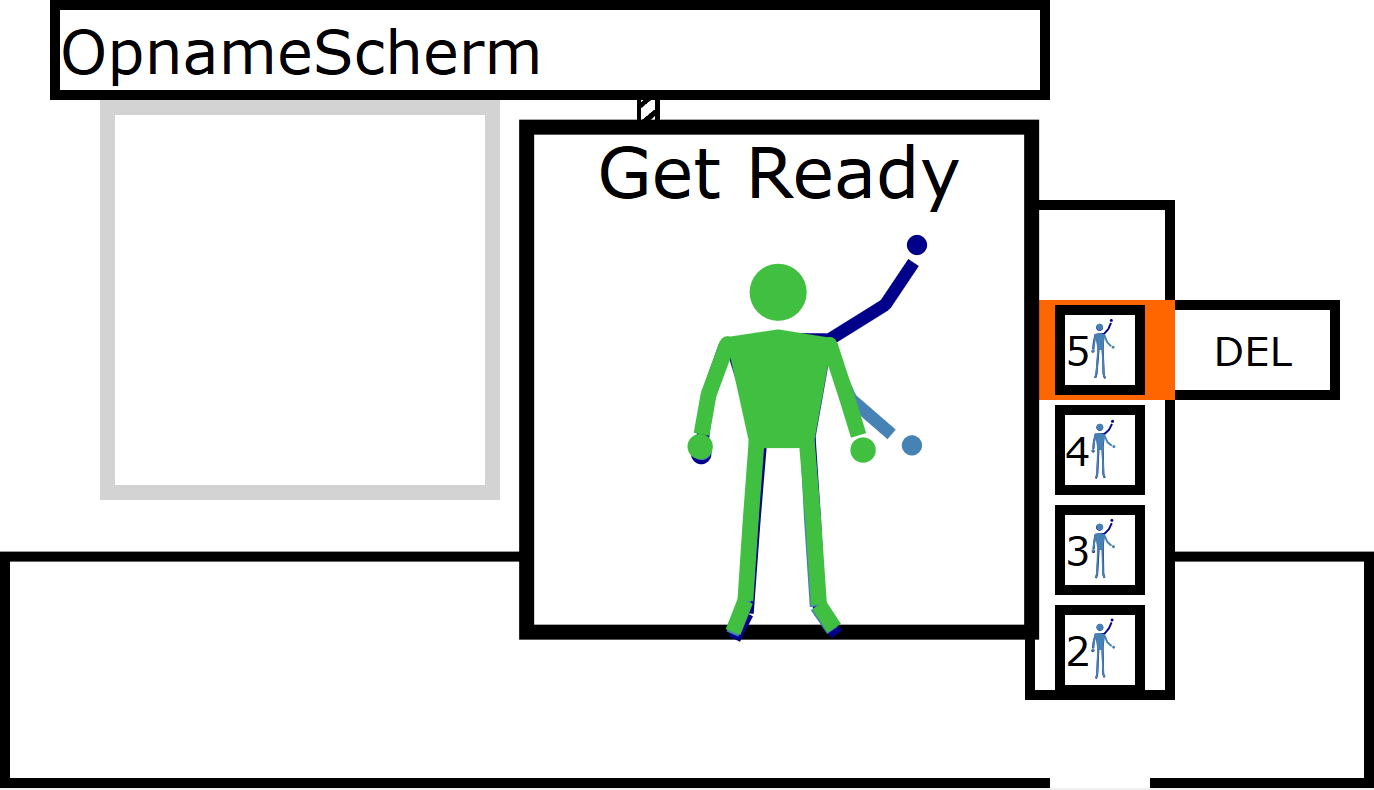
\includegraphics[width=16cm, height=9cm]{figures/4_record_getready.png}
		\caption{\emph{First view of the recording screen}}
		\label{The regular view of the end desing of the UI}
	\end{center}
\end{figure}

\begin{figure}[H]
	\begin{center}
		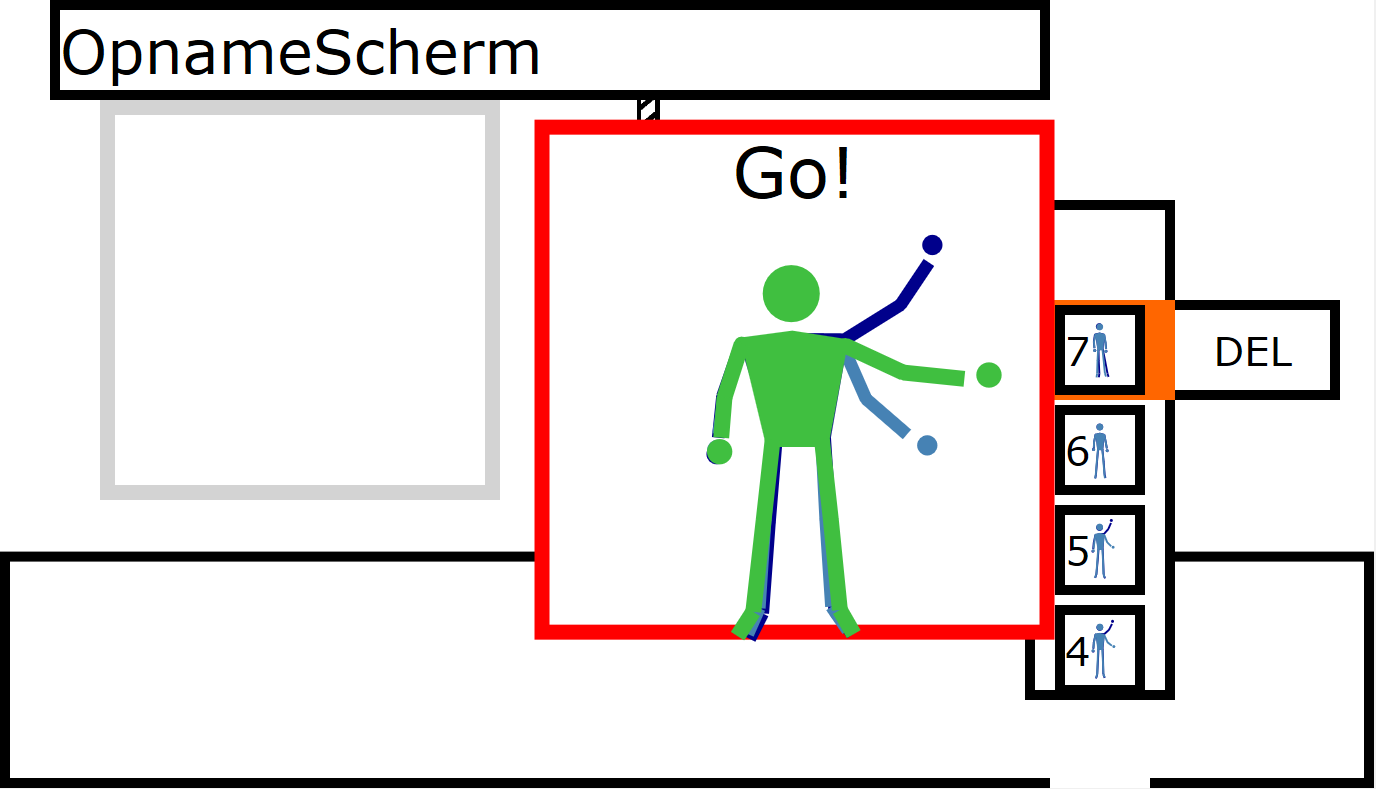
\includegraphics[width=16cm, height=9cm]{figures/6_record_start.png}
		\caption{\emph{View when the program starts recording, between this and the first view there is a countdown from 3, after the user stands still for a certain amount of time to text in the window will read "Done!"}}
		\label{The regular view of the end design of the UI}
	\end{center}
\end{figure}

As said before the scrollbar contains elements that are each linked to a recording of the current exercice. In these boxes a small preview can be seen of the start and end position of the linked recording in the same color scheme as during recording. The numbering of the boxes goes from the first recording as one counting up to the last recording, though these numbers are not the same as the ID's of the gesture class as seen further on during the discussion of the backend but the order of the numbers is still the same. When the user hovers one of his hands over the recorded element within the orange area the effects as seen in \textbf{ fig 8} are triggered. The the specific recorded element is replayed within the previously grayed out window on the left. The blue bar on the bottom of the window indicates the progression of the recording. As long as the user hovers over the element in the scrollbar the recording is repeated with half seconds delays between repeats. This was a deliberate choice to make sure the user is fully aware of which recording is playing in the window, he should notice that the recording is only playing when he touches it. For the same reasons the number of the recording is also displayed on the left of the screen where it does not obstruct the user in reviewing his recording but is there when the user is uncertain of which recording is playing. Additionally both the orange selectionbox in the scrollbar and the edges of the display screen are colored green, the color previously linked with hover over information. The emphasizes on clearly linking the replay with the recording comes from the fact that the screen is so far from the actual element it is connected too. The scrollbar is on the right because it is easier to operate for right handed users which is more likely to be the case and the delete action is already on the right of it and can hardly be moved for reason given later on. Following both the proximity and similarity law of the Pragnanz law's would make the most sense but placing the screen on the right of the delete button would still have the delete button between it and the recorded element and would place the user's puppet to far from the center of the screen, out of the focus of the user.\\

\begin{figure}[H]
	\begin{center}
		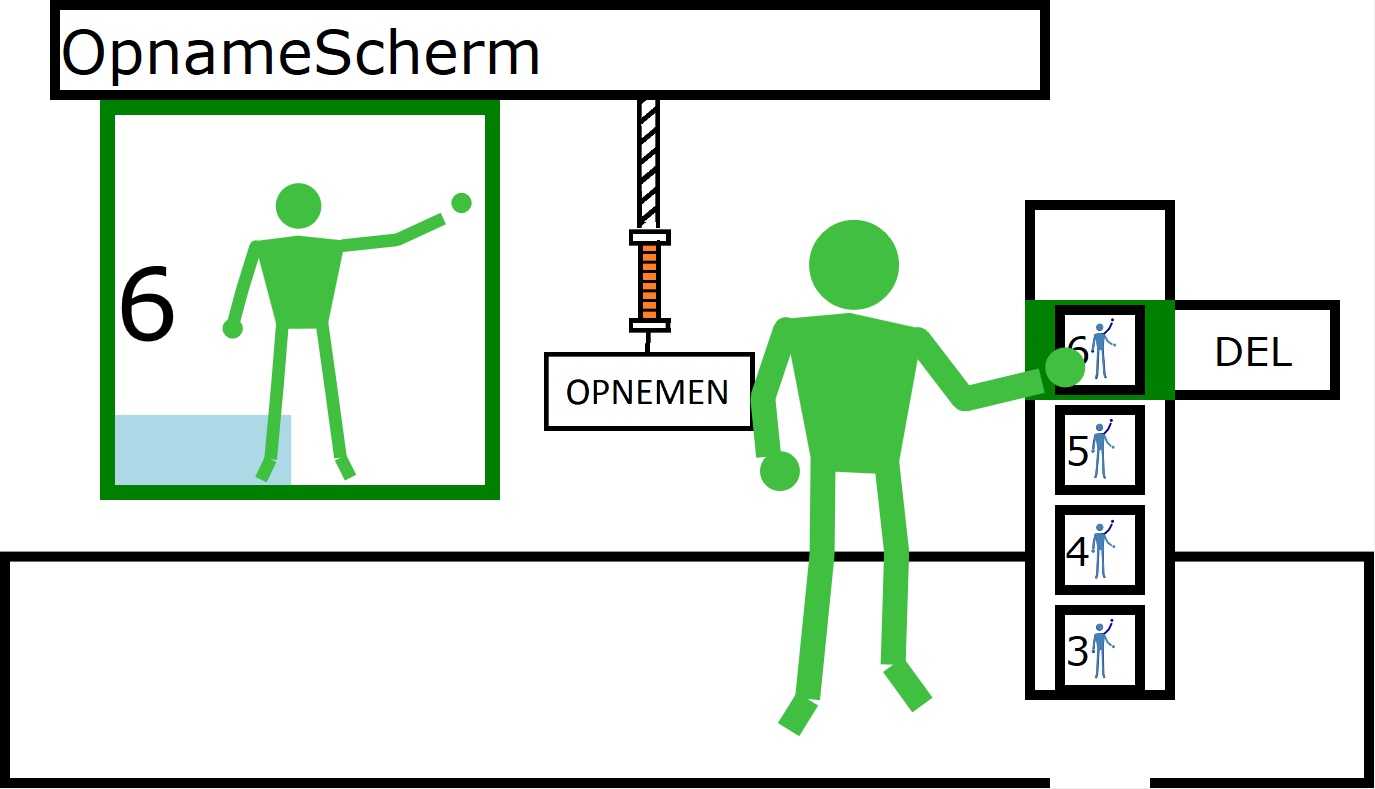
\includegraphics[width=16cm, height=9cm]{figures/11_replay_recording.png}
		\caption{\emph{The recorded element six is replayed to the user by hovering over it with any hand.}}
		\label{replay of element six}
	\end{center}
\end{figure}

To activate the scroll function on the scrollbar, the user has to hover his hand within the boundaries of the black bordered box but not within the orange selectionbox, the black borders of the scrollbar turn green to indicate that the user is hovering over the scrollbar, this is shown in \textbf{ fig 9}. Scrolling is only starts when the user has moved a small distance up or down to avoid to scrollbar being immediately stuck to the user which would be annoying. Onces scrolling is started it continues as long as the user keeps moving in the same direction, this also counts when going through the selectionbox area and even when going outside of the scrollbar's borders. This makes sure that the user is not surprised by as sudden stop of the scrolling action when accidentally going inside of the selectionbox or outside of the scrollbar. The whole reason why the user cannot initiate a scroll within the selectionbox is because the element that is placed there has to be able to be hovered over to display it, as explained earlier and it has to be able to be moved to the side for deletion. Accidental activation of the scroll function is minimized by this measure. Though there is more to this, informal tests with user that are not familiar with the UI often tried to scroll down or upward starting from the selectionbox, the activation of the scroll function only after the user left the selectionbox area proved to confuse the user. To counter this the activation area of the scroll function is expanded into the orange area for about 15 percent of the selection box height on both the top and the bottom. Once activated the element stay on a fixed distance from each other but all elements are moved with the same dynamics as used in the record rope, they perform the same relative movement as the hand that is hovering over it. During scrolling all recorded elements are locked to any interactions and the element that will land in the selection box is indicated by a light blue coloring of the white background. The example of scrolling can be seen in \textbf{ fig 10}. When the user stops scrolling the recorded elements are locked into positions as seen in \textbf{ fig 9}. Only the element in the selection box can be interacted with.\\

{\large COMMENT: talking about how why using the slide with a closed hand is a bad idea} \\

\begin{figure}[H]
	\begin{center}
		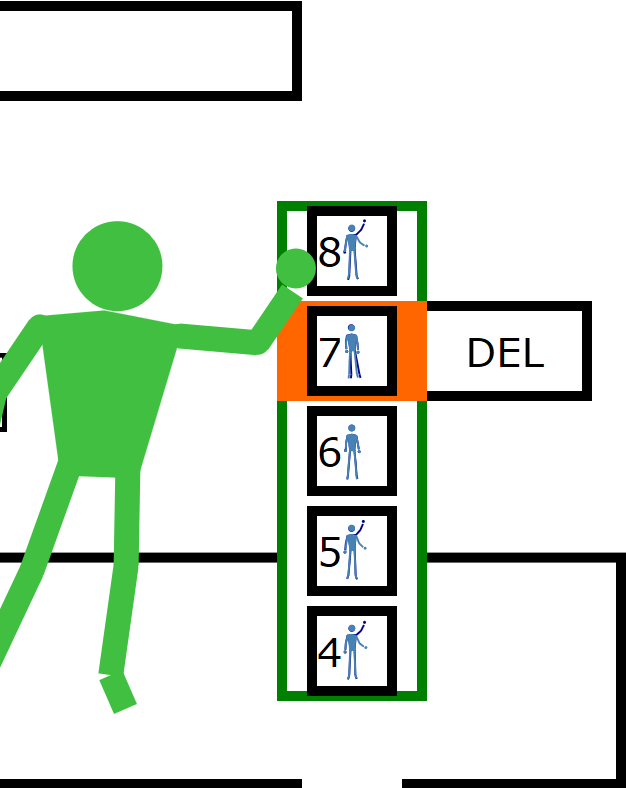
\includegraphics[width=6cm, height=8cm]{figures/9_hover_scrollbar.png}
		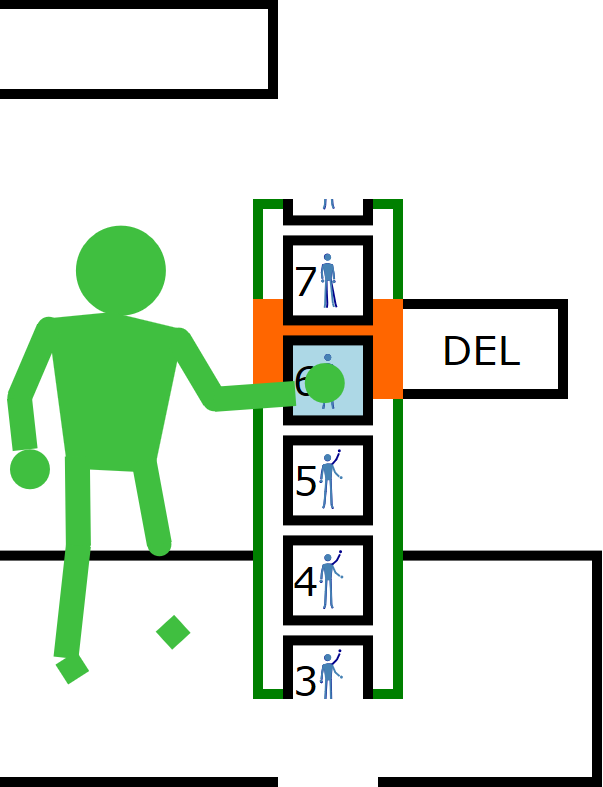
\includegraphics[width=6cm, height=8cm]{figures/10_scroll_scrollbar.png}
		\caption{\emph{Reaction of the scrollbar: a) when hovered over, b) when scrolling is activated}}
		\label{The regular view of the end desing of the UI}
	\end{center}
\end{figure}

The delete sequence of the recorded element in the selection box can be started by hovering over the middle of it. After this the element will follow the relative horizontal movement of the interacting hand between start point and end point with the same dynamics as the scrollbar and the rope. As seen in \textbf{ fig 10}, The "DEL" box is filled up with a red bar to indicate how far the user still has to move until the item is deleted. When the end point is reached the recorded element turns red and fades away within a halve second to clearly indicate that this recording is deleted. Once the endpoint is reached the action is irreversible and for the duration of the fading the scrollbar and all the elements are locked for any further interaction. An example of this is shown in \textbf{ fig 11}. The reason why this action is only started from the middle is to increase the difference between initiating the delete sequence and replaying the recording and also heighten the threshold to start such a serious action as deleting an item. After deleting an element the other recorded elements are renumbered.

\begin{figure}[H]
	\begin{center}
		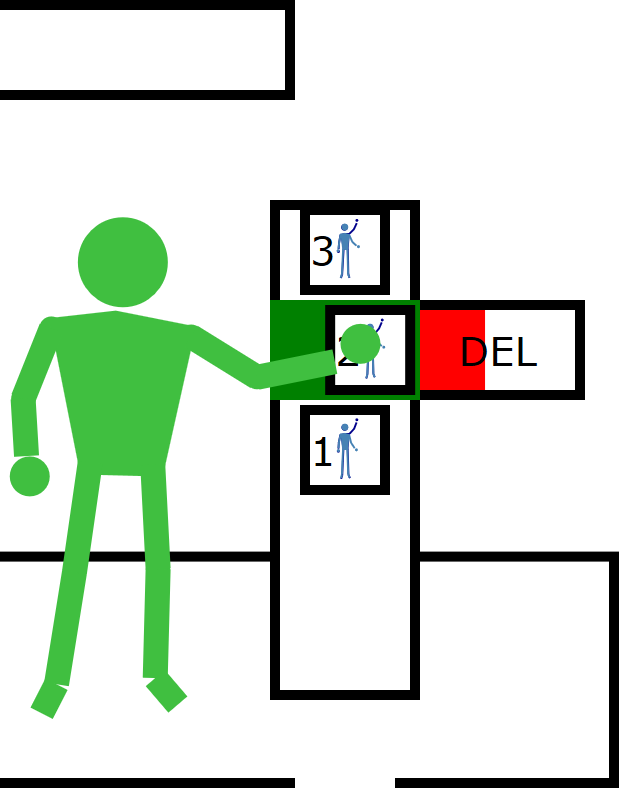
\includegraphics[width=6cm, height=8cm]{figures/12_delete_progress.png}
		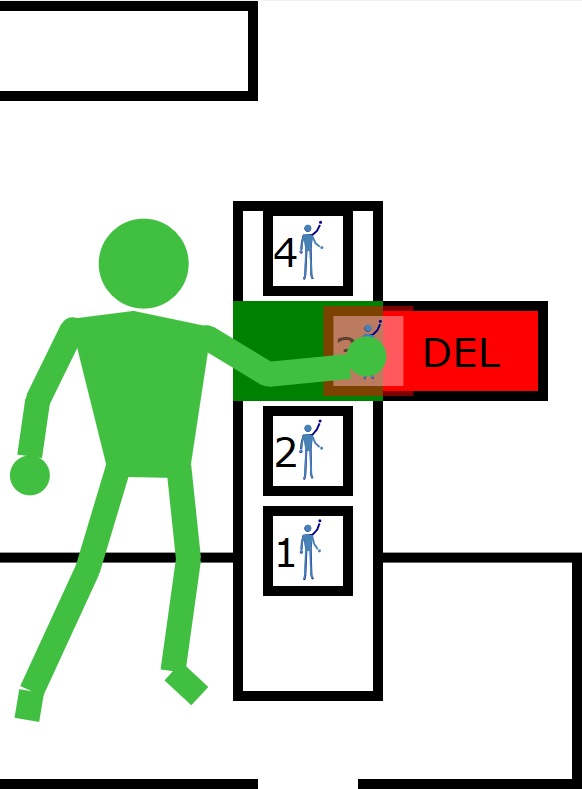
\includegraphics[width=6cm, height=8cm]{figures/13_delete_complete.png}
		\caption{\emph{The delete sequence: a) the user in the process of deleting, the red progress bar indicates how far until deletion the user has to go , b) The endpoint of the action is reached, the item turns red and fades after which it is deleted}}
		\label{The regular view of the end desing of the UI}
	\end{center}
\end{figure}



%TODO beschrijving + afbeeldingen van de uiteindelijke interface

\subsection{Software}

\begin{figure}[H]
\begin{center}

\includegraphics[width=8cm]{KUL.png} %PLACEHOLDER, CHANGE THE FILENAME
\caption{\emph{The class diagram of the application, focusing on the GUI}}
\label{fig: gui_classdiagram}
\end{center}
\end{figure}

%TODO klassendiagramma van de GUI + eventuele snippets uit de code (+ uitleg)


\section{Back-end software}
\label{section: Back-end software}

The focus of the application is reflected by the structure of the code. The class diagram shows a model-view pattern do make a distinction between the graphical interface of the application and the back-end (see figure \ref{fig: backend_classdiagram}).\\

\begin{figure}[H]
\begin{center}

\includegraphics[width=8cm]{KUL.png}
\caption{\emph{The class diagram of the application, focusing on the back-end}}
\label{fig: backend_classdiagram}
\end{center}
\end{figure}

The Kinect camera has the ability to identify and measure the position relative to the camera of 25 points of a person, for instance: left elbow, right elbow, head, center of the spine, left wrist,\ldots All of these points are referred to as \classname{Joint}s and can be accessed using the libraries that come as part of the Kinect SDK installation. Each \classname{Joint} has an $x$, $y$ and $z$ coordinate, so it is unambiguously defined in space.\\

When the Kinect measures all of the \classname{Joint}s at one specific point in time, these 25 \classname{Joint}s together form one frame. This can be seen as a single picture of a person taken by the camera. Analogous to a movie, which is nothing more than a quick succession of pictures, an instance of \classname{Gesture} collects all \classname{Frame}s, which all together, contain information about how the person moved over a period of time.\\

In order to improve the application's ability to recognize an exercise, each of the exercises must be trained more than once by the physical therapist. For each exercise that is trained, an instance of \classname{Gesture} is created. The \classname{Gesture}s that contain data about different executions of the same exercise are grouped into a \classname{GestureClass}. In other words, one \classname{GestureClass} object contains all trainings of the same exercise.\\

After setting up a \classname{Project} object, it contains all data that is needed for playing a game using the application. It has a \classname{map} that maps a label for each exercise to a \classname{GestureClass} and the actions linked to that \classname{GestureClass}. An \classname{Action} contains information about the keyboard key that needs to be pressed and if that key should be held down or be quickly pressed and released. The \classname{Model} class forms the core of the application. It controls the flow of the program and contains all important objects, such as the \classname{Project} and the \classname{GestureClass}es.\\

%SOURCE FOR LIBSVM REQUIRED
\classname{SVMInterface} takes all gesture data and converts it to a format that is accepted by the LibSVM library. This is an existing library that provides a C$++$ support vector machine implementation used for gesture recognition.\\

To prevent having to train all exercises again each time the application is started, all necessary data is saved into files in the data folder using the \classname{Filewriter} implementation. This includes the data of the \classname{Gesture}s, \classname{GestureClass}es, \classname{Project} and the computed SVM model. The \classname{Filereader} is responsible for reading data from the saved data files when the application is started.


\section{Gesture recognition}

\subsection{Support vector machine}

In order to provide enough flexibility concerning the type of exercises, SVM is used. SVM supports supervised machine learning and its use encompasses two modes: train and predict.\\

A model can be trained with a given set of data and a label to classify the gesture. The amount of numbers in one data set is referred to as the number of features. If it contains $n$ features, the entire data set can be seen as a single point in a $n$-dimensional space. It is possible to train the same gesture more than once. In that case, the same label is used to indicate that the given data set is related to the same gesture. In other words, all trainings of the same gesture are linked to the same label. All of these trained gestures with the same label are seemingly similar, but actually contain variations due to noise during the measurement of the gesture or a slightly varying execution of the gesture.\\

After training all required gestures, a SVM model is created. Given a data set of a gesture, this model can predict which of the trained gestures has the biggest resemblance to the given data set. As a result, the label of the most similar trained gesture is returned. This also explains the necessity of having multiple trainings recorded for each gesture. Errors in a single training due to noisy measurements of the Kinect camera can lead to wrong predictions. Having multiple trainings minimizes the influence noise has on the prediction and keeps into account that the user executes all gestures with slight variations. As a result, the model can predict more accurately which gesture is performed.\\

However, there are some things to keep in mind when applying this strategy. Firstly, while inputting multiple repeats of the same gesture helps with predicting the gesture after a model is created, it takes more time for the therapist to do this. Secondly, when trying to predict a gesture, the generated SVM model always returns the label of the most similar gesture, even if they are not related at all.\\

These problems are tackled as part of the approach to using SVM to predict gestures.


\subsection{Approach}

As stated in section \ref{section: Back-end software}, a gesture consists of multiple frames. Each frame contains 25 joints and each joint consists of an $x$, $y$ and $z$ component. This results in a total of 75 features that are being considered for each frame.\\

Two approaches are considered when it comes down to learning how to recognize gestures. By directly comparing these approaches, it is easier to identify their advantages and disadvantages.\\

The first approach is to add a time stamp to each frame as an extra feature, which indicates the time relative to the first frame of the gesture. This results in having 76 features per frame. If performing a certain gesture takes about $t$ seconds and is captured at a rate of $f$ frames per second, this amounts to 76 $tf$ features. This additional feature can be used to make sure that the gesture isn't just similar in space, but also in time. For a 3-second gesture recorded at 30 frames per second, which is the highest sampling speed of the Kinect camera, this amounts to 6840 features for a single training of the gesture. In other words, the number of features of one training depends on the duration of the gesture. The entire gesture is classified as a single gesture. During prediction, a gesture with the same number of features can be input to verify if that gesture matches any of the trained gestures.\\

There are several problems with this first approach. If the number of features of the gesture used for predicting does not match the number of features of the training gestures, the prediction is not accurate and should be discarded. Discarding is necessary as SVM always returns the label of a gesture, even if the predicted gesture is completely unrelated to any of the trained gestures. This poses a problem as different gestures can have a different duration. Even different trainings of the same gesture can take for instance 3 seconds and 3.1 seconds, implying that the recordings have a different number of frames and thus a different number of features. A possible solution is to recalculate the entire gesture and use interpolation to convert the set of frames to a new set with a known, fixed size and preferably with equidistant time stamps.\\

Furthermore, not just the trainings of one gesture, but all of the gestures need to have the same number of frames. The gesture to predict is not known beforehand and can only be predicted accurately if the number of features for both the predicted gesture and trained gesture are equal. As a result, it is required that all gestures have an equal amount of features. This means that short gestures need to be mathematically extended with additional frames to match the size of longer gestures. Another side effect is that all gestures need to have the same duration, not just the same amount of features. This limits the therapist in choosing exactly what exercises he wants the patient to perform. Also, predicting a gesture can only be as fast as the trained gesture with the longest duration. More in particular, assume the longest gesture is 5 seconds in length. It then follows that it takes about 5 seconds to predict any gesture. This also means that patients that control the game can only perform one action every 5 seconds. As the games to be played are unknown beforehand, a slow reaction time of the application can render some games unplayable. As such, this approach is not viable.\\

The second approach is to split up one gesture into $n$ smaller gestures and classify each of them differently, assigning a different label to each part of the gesture. Assume that a gesture is split up into 4 smaller parts so that each part contains approximately an equal amount of frames. Consider a 4-second gesture sampled at 30 frames per second. The complete gesture consists of 120 frames. By splitting it up into 4 parts, each part contains 30 frames. All first 30 frames are labeled with the same label, for instance 1. The next 30 frames receive a label 2, and so on. To put it differently, the considered gesture is split up into 4 postures with each having 30 slightly varying trainings. In contrast to the first approach, as described above, prediction does not happen for an entire gesture, but for separate postures. The condition for having executed the entire gesture is that each of the postures are predicted correctly and in the right order. To put it differently, $n$ \emph{pictures} are taken of the gesture and if at some point during prediction all pictures are executed in the right order, the application acknowledges the execution of the gesture.\\

AFBEELDING NODIG MET EXTRA UITLEG IN ALINEA HIERBOVEN\\

The biggest advantage of this approach is the flexibility of it. Each posture corresponds to a single frame, which contains 75 features. This eliminates the need of having gestures with the same length or having to modify training data to have gestures with an equal number of features. It is even possible to not just link a gesture, but also a posture to a keyboard button, which allows the physical therapist to choose the exercises that fit the needs of a patient the best. Additionally, the application reacts immediately to an executed gesture, not after a fixed amount of time. This allows for a wider variety of games being playable using this application.\\

Another advantage is that it solves the issue where SVM always returns the label of a predicted gesture, even when the patient is not doing anything. A gesture is only recognized when all parts of it are executed. In other words, gestures are not recognized involuntarily and, as such, actions like button presses that influence the game are not executed by accident. This also means that no neutral or \emph{wrong} gestures are required to link a certain gesture to no in-game action.\\ %TODO verduidelijken

The disadvantage of this second approach is that there is no strict requirement for the entire gesture to be executed in about the same time as the gesture recorded during training. If a gesture is executed faster during prediction compared to during training, it is recognized as the same gesture being executed. However, it is possible to solve this timing issue to some extent when the gesture during predicting is performed slower. The gesture can be ignored if more than a certain amount of time passes. This time threshold takes the gesture with the longest duration into account and is chosen higher than this in order to allow all gestures to be executed and successfully recognized.
\chapter{Implementation}

\begin{itemize}
\item Bespreking van werking van belangrijkste softwareonderdelen
\item Belangrijkste deel/delen uit code
\item \ldots
\end{itemize}


\section{Requirements of the application}

The application is developed in C$++$ using Microsoft's Visual Studio IDE and can run on computers with a Windows operating system. On an implementation level, platform-specific features are used for saving and loading data files and running the GUI. On a hardware level, the Kinect 2.0 camera requires the installation of a driver in order to function properly. This comes as part of the \emph{Kinect for Windows SDK 2.0}. Microsoft's download page states the system requirements for using the Kinect 2.0 camera. These requirements are: 64-bit processor, dual-core 3.1 GHz or faster processor, USB 3.0, 4 GB of RAM or more, graphics card that supports DirectX 11, Windows 8 or 8.1, Windows Embedded 8 or Windows 10.\\

The application, including resources like images, takes up approximately 20 MB. Saving all exercises needed for playing a game takes up approximately 0.6 MB. This depends on the number of exercises recorded, the number of trainings for each exercise and the duration of each exercise. 


\section{Graphical user interface}




\section{Back-end software}

\begin{lstlisting}[caption=the controlling method that is part of the back-end's main loop, label=code_process_body]
void Model::processBody(INT64 nTime, int nBodyCount, IBody ** ppBodies) {
	//Go through all the bodies that are being seen now. If a body is tracked, its frame is made and added to the frames vector
	for (int i = 0; i < nBodyCount; ++i) {
		pBody = ppBodies[i];
		if (pBody) {
			bool bTracked = false;
			HRESULT hr = pBody->get_IsTracked(&bTracked);

			if (currentActiveBody == -1 && SUCCEEDED(hr) && bTracked)	//No body is tracked at the moment {
				currentActiveBody = i;
			}

			if (SUCCEEDED(hr) && bTracked && i == currentActiveBody) {
				Frame relFrame(pBody);					//Create a frame of every tracked body
				Frame absFrame(pBody, false);

				relFrames.push_back(relFrame);
				absFrames.push_back(absFrame);
				
				if (recording) {
					recordGesture(relFrame);
					break;
				}

				framesBuffer.push_back(relFrame);

				if (refresh && !predict) {		//The measure button was pressed last
					updateCountDown();
				}

				if (predict) {
					if (!trained)	{			//If the model is not yet trained, train it
						train();
						trained = true;
					}
					int label = SVMInterface::test(activeProject->getSVMModel(), relFrame);
					addToLabelsBuffer(label);
					predictAndExecute(label);
					view->setPredictedLabel(label);
				}
			}
			else if (i == currentActiveBody) {				//If the current tracked body is lost for this frame
				bodyLostCounter++;											//Increment the lostBodyCounter
				if (bodyLostCounter > BODY_LOST_LIMIT) {//If the limit is reached, reset the currentActiveBody
					currentActiveBody = -1;
					bodyLostCounter = 0;
				}
			}
		}
	}

	if (updateUI) {
		view->updateHitboxes();
		updateUI = false;
	}
	displayFrames();
}
\end{lstlisting}


\section{Gesture recognition}

It is possible to split up the implementation of gesture recognition in two parts: the recording of a gesture by the physical therapist and the prediction of a gesture executed by a patient.


\subsection{Recording a gesture}

\begin{lstlisting}[caption=method to record a gesture, label=code_record_gesture]
void Model::recordGesture(Frame & frame) {
	if (!initialized) {
		frameNeutral.setFrame(frame);
		initialized = true;
	}
	
	framesBuffer.push_back(frame);

	if (!startedMoving) {
		if (! frame.equals(frameNeutral)) {
			startedMoving = true;
			framesBuffer.clear();
		}
		else if (framesBuffer.size() > NOT_MOVING_FRAME_DELAY) {
			addRecordedGesture();
		}
		else {
			return;
		}
	}

	if (framesBuffer.size() > NOT_MOVING_FRAME_DELAY &&	framesBuffer.back().equals(framesBuffer.at(framesBuffer.size() - NOT_MOVING_FRAME_DELAY))) {
		addRecordedGesture();
	}
}
\end{lstlisting}


\subsection{Predicting a gesture}

Code snippet \ref{code_gesture_executed} shows a piece of code.

\begin{lstlisting}[caption=method to verify if a gesture with given label is executed, label=code_gesture_executed]
bool Model::isGestureExecuted(int checkLabel, int posInBuffer, int recursiveCounter, int badCounter) {
	//The label exists and is linked to a posture.
	if (activeProject->containsLabel(checkLabel) && activeProject->getGestureClass(checkLabel)->getGestures().front()->isPosture())
		return true;

	//Done enough recursive checks to confirm the gesture has been executed.
	if (recursiveCounter >= NB_OF_LABEL_DIVISIONS)
		return true;

	int nextLabelToCheck = checkLabel - 1;
	for (int i = posInBuffer; i >= 0; i--) {
		if (labelsBuffer.at(i) == nextLabelToCheck)
			return isGestureExecuted(nextLabelToCheck, i, recursiveCounter + 1, 0);
	}

	//If this point is reached, a label that is one less than the given
	//	label cannot be found in the buffer.
	//The gesture may still have been executed, so keep checking for the
	//	next one if the badCounter is not too high.
	if (badCounter > 0)
		return false;
		
	return isGestureExecuted(nextLabelToCheck, posInBuffer, recursiveCounter + 1, badCounter + 1);
}
\end{lstlisting}
\chapter{Results}

Usability tests make it possible to verify if the design meets the expectations of the target group and offer a way to discover unexpected problems that are hard to track by the developers themselves. Test persons have a fresh look on the application and can provide useful insights in the way they interpret visual elements of the user interface.\\

In addition, the technical evaluation considers the effect of the implementation, ensuring that the user is not hindered by performance issues or similar problems.


\section{Usability test}

The graphical user interface is designed for use by physical therapists. As such, acquiring feedback from therapists is essential in developing an interface that is both useful and easy to use. The process of the usability test is described, followed by an overview of the most important results of the evaluation itself and an interpretation of these results.


\subsection{Description of the test}

A usability test is conducted with physical therapist Dries Lamberts at Windekind Leuven, an organization that focuses on the education of children with disabilities and offers a full program to assist them with their specific difficulties. For this test, the Kinect camera is connected to a computer that runs the application and, positioned on a desk at hip height. The user indicates that he is familiar with using the Kinect camera and motion-based games.\\

A short introduction on the purpose of the application is given to the test person for reference. After that, he is presented with several tasks and is asked to apply the think-aloud protocol in order to obtain as much information as possible about the interaction with the application and the thoughts of the user while doing so.\\

In preparation of the usability test, gestures are pre-recorded that both serve the purpose of testing the robustness of the application as well as having a fallback plan in case problems arise during the test.\\

One task is to watch the pre-recorded gestures and control a game called Space Invaders using the pre-recorded gestures. This is a game that has an avatar move left or right on the screen and shoot bullets (see figure \ref{fig: space_invaders}). As such, four gestures are pre-recorded: one gesture that allows the avatar to move to the left, one to move to the right, one to shoot bullets and a neutral gesture that is linked to no keyboard key. At this point, it is explained to the user that a neutral gesture is required in order to have a gesture to which no keys are linked. This is explained without going into detail about the specifics of SVM. The goal of this task is twofold. Firstly, the task is used to verify if the test person is able to watch replays of the pre-recorded gestures without any guidance and to learn what gestures are pre-recorded without additional information. After this is done, it is explained to the user how the gestures and keyboard keys are linked together. Secondly, it makes it possible to confirm if a correct prediction of a gesture execution does not depend on the person performing the gesture, as problems can arise due to the person recording the gestures and the person playing a game having a very different physique.\\

\begin{figure}[H]
\begin{center}
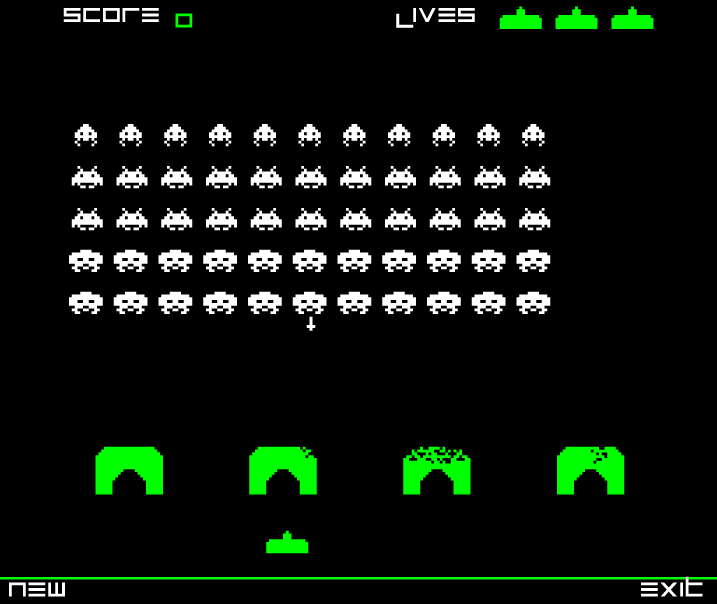
\includegraphics[width=8cm]{SpaceInvaders.png}
\caption{\emph{Screenshot from Space Invaders}}
\label{fig: space_invaders}
\end{center}
\end{figure}

Another task is to play the game Sokoban Geek. This puts the gamer in control of an on-screen avatar that can move up, down, left or right. Walking into boulders allows the player to move them in order to solve a puzzle (see figure \ref{fig: sokoban_geek}). The game is shown to the test person and after trying the game, he decides how many gestures are required to play the game. Then, he comes up with different gestures for each input and records three trainings for each of them. The test person is asked to delete a recorded gesture and record it again. After recording all gestures, he tries to play the game. The goal of this task is to check how the test person reacts to the recording elements of the interface and if it is clear how to interact with them without assistance.\\

\begin{figure}[H]
\begin{center}
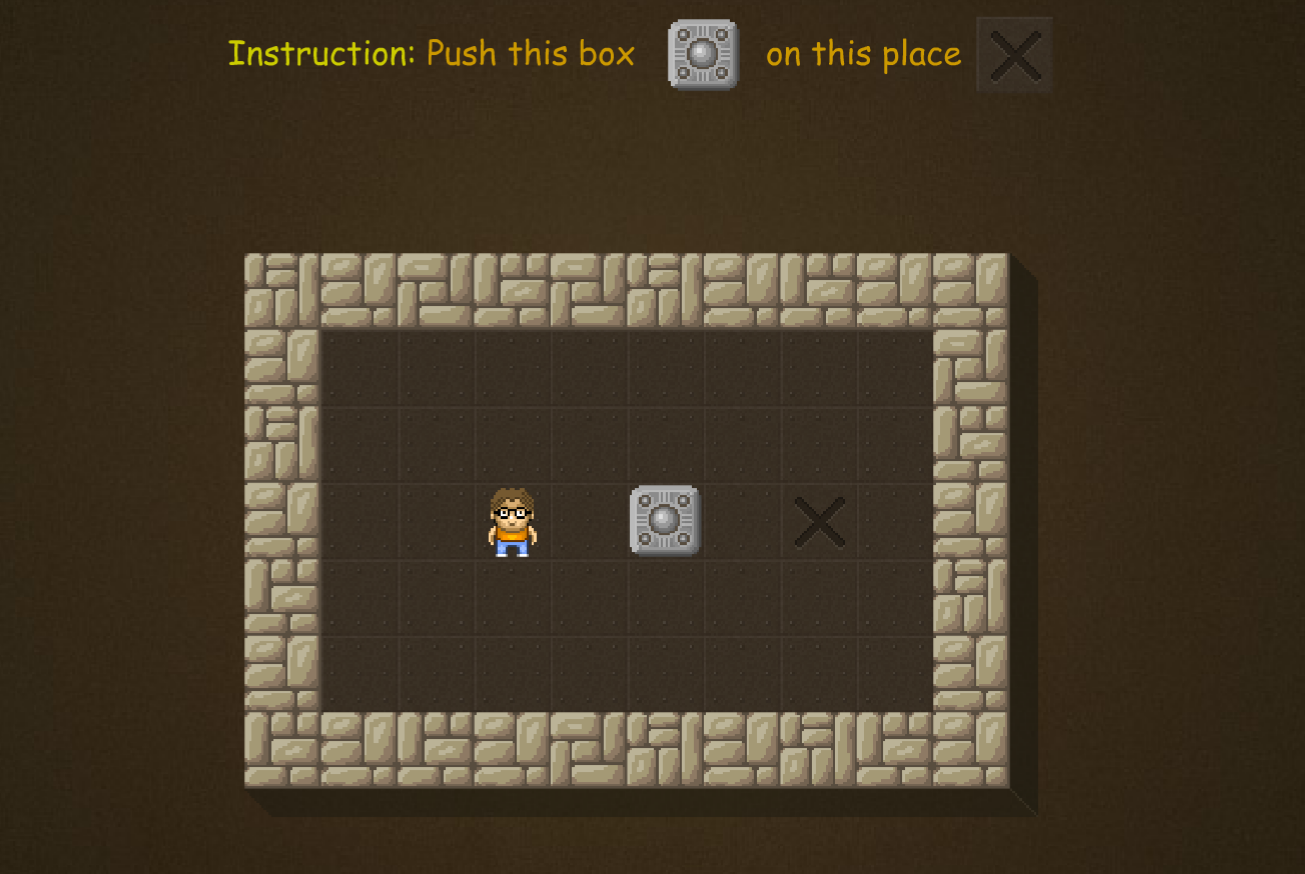
\includegraphics[width=8cm]{SokobanGeek.png}
\caption{\emph{Screenshot from Sokoban Geek}}
\label{fig: sokoban_geek}
\end{center}
\end{figure}

With permission of the test person, during the entire test, the computer screen is recorded, as well as everything said, for analysis purposes. The system usability score (SUS) allows to obtain a numeral indication of the usability of the application based on ten questions. At the end of the usability test, the user is asked to fill out a questionnaire with these ten questions. While this score gives an indication of the application's usability, it is not possible to draw firm conclusions as a larger number of test persons is required in order for the usability score to be statistically relevant.


\subsection{Results}

This section will describe how the physical therapist interacted with the UI that was seen in chapter \ref{interface description}, there all the figures to which this section refers are shown.

For the first task, the user notices the recorded gestures in a list on the right-hand side of the screen. By trying to move its avatar's hand to align with the previews of the recordings, he notices that it is possible to scroll through the list of recordings. He also notices the delete option next to the recordings list and indicates that he is anxious about deleting one of the recorded gestures because of the rather aggressive red color of the progress bar.\\

Watching a replay of the recorded gestures initially is not clear to the user. He tries to drag one of the gestures to the square on the left hand-side of the screen, which is intended to be the display screen. He notices that this is not possible, but makes several attempts do this. After that, he indicates that he can't find it and looks at the interface without trying to interact with anything. To replay a recorded gesture, the user can point with the avatar's hand to the recorded gesture in the orange area of the scrollbar, previously referred to as the selection box area. At that point, a replay of that gesture is displayed automatically. The replay stops while scrolling through the list or when not pointing at the gesture in the selection box area. The user did this several times during this task subconsciously, without noticing that a replay started playing at the left side of the screen. A factor adding to this problem is the fact that the recordings were displaying a posture rather than a gesture, which in fact is a static image instead of an animation. The user required assistance to complete this task. He was able to do this after knowing that the gesture in the selection box area is displayed at the left-hand side square.\\

After watching replays of the recorded gestures, the user is able to replicate in real life what gestures are recorded and displayed on-screen. When the Space Invaders game is started, the user has no problem interacting with the game and does not require any assistance. He is able to control the in-game avatar subtly and meet the game objectives. After asking for his experience with the controls, he indicates that the controls are responsive and that he does not experience any lag.\\

For the second task, the user gets the chance to see what the Sokoban Geek game looks like and how it is played. After that, he states that he needs five gestures to play the game. Four gestures are linked to a directional keyboard key and one gesture that serves as the neutral gesture. To record a gesture, it is required that the user hovers the hand of the on-screen avatar over the grip of the pulling cord, makes a fist, and move his fist down to start recording. This translates to pulling the displayed cord. When trying to start recording the first gesture, the user pulls the cord without any problems. The recording screen appears and he starts performing a gesture when the interface indicates that recording has started. He stands still when he is done with the gesture and the recording stops automatically.\\

Upon being asked to delete the gesture he just recorded, he needs no assistance to push the gesture object to the right into a box indicating that the gesture can be deleted. He indicates that his earlier anxiousness of deleting a gesture by accident is unnecessary, as it requires some effort to perform this deleting action and it is hard to do it by accident.\\

When trying to record a gesture the second time, the user is unaware that he is required to close his hand into a fist to pull the cord. He tries hovering over the grip and moving his hand down and indicates that he isn't sure why recording does not start this time. Only after several tries, he tries closing his hand to pull the cord, activating the recording screen. He states that he did not know that closing the hand was required and that he did that by accident to record the first gesture. He indicates that he has experience using the Kinect camera for other games and that these games never required to close a hand, so he was unaware that the Kinect is able to make a distinction between open and closed hand.\\

The user notices clearly that the recording of a gesture stops when he stands still. Because he was not aware of this, one gesture was not recorded the intended way, but the user was able to delete this gesture and record a new one without assistance. The user also noticed that the light blue and dark blue puppets behind his puppet during the recording screen indicate the beginning and ending position of his first gesture. He states that this feature is very useful for repeating the original gesture.\\

When trying to watch a replay of a recorded gesture, he is not sure if he needs to point at the gesture with open or closed hand. Although both cases function in the same way, the user states that using a closed hand feels like the application responds better. He also wondered whether the recording would distinguish the difference between open and closed hand, but concludes that it does not because the replay of the recording does not show any difference. This is as intended. While watching the replay, he noted that it is not possible to accurately tell what a gesture looks like when stretching for instance an arm straight ahead. The replay does not provide any information about depth.\\

After the user records all gestures, he is able to play the game. However, the gesture that is linked to the left arrow key does not respond. The user is asking if the key is linked correctly to the gesture and thinks this is the problem. He misses feedback about what gesture is linked to what key, though it should be noted that the concept is that keys would be assigned on a different screen in a full application. After verifying for the user that the key is linked correctly, we present him with the question of how he would handle this problem without any assistance. He suggested to delete the recorded gestures and record them again. After doing this, the user is able to play the game without further problems. Analogous to the situation of playing the first game, the user plays the second game with similar ease.\\

The entire user test approximately took 45 minutes. After the test, the user asked because of his own experience with disabled children if very small gestures are supported by the application and if the application can be used for other purposes than playing games. An example he thought of was using gestures to type words using sign language. He also added that he was glad that use of the space bar is supported by the application, as he has experience with similar projects that do not support the space bar, while it is one of the most used keys in computer games. However, a lot of games the children are interested in require the ability to point with a cursor on-screen. This is a feature he would appreciate. Finally, he stated that he is very interested in using the application, allowing disabled children to play games and exercise while doing so.


\subsection{Discussion}

The physical therapist proved to understand the concept of the application. This shows that it is possible for persons without programming knowledge to use the application for recording gestures and controlling computer games. He also understands that the use of the application is not limited to games and can also be used for other computer applications that require keyboard input.\\

A few tries are required to get familiar with how to start recording and how to end it. In particular, without prior knowledge or experience, more feedforward is required to communicate that the hand needs to be closed when pulling the cord and that the user needs to stand still to stop recording. However, after a few tries, it is possible to record multiple gestures in succession without any of them not being recorded as intended.\\

Replaying recorded gestures requires the user to align his on-screen hand with the gesture inside the selection box area of the scrollbar. There is no form of feedforward indicating that performing this action results in the gesture being replayed. The feature is intended for the user to be discovered while scrolling through the gestures or while trying to delete a gesture. As such, this can be confusing to the user.\\

Both the actions of recording gestures and replaying recorded gestures are performed faster after having experienced this firsthand. The provided feedforward is too subtle to immediately make it clear what actions are expected. To improve this, it is either possible to provide more explicit feedforward, or to introduce the user to the most important functions using a tutorial.\\

When playing the games using gestures, the test person appears to be very engaged in them and the way they are controlled. This is an indication that not only the application succeeds in its purpose of playing a game with gesture-based input, it also can make for a pleasant experience.


\section{Technical evaluation}

The application is developed with the Microsoft Visual Studio integrated development environment (IDE) in C$++$ and can run on Windows operating systems. This limitation is due to the use of the IDE's visual interface editor and Direct2D, as well as the feature of saving and loading data files. The application is tested to run on both Windows 8.1 and Windows 10 machines.\\

All of the required files for running the application, including resource images, take up approximately 20 MB of space. Saving all gestures needed for playing a game takes up approximately an additional 0.6 MB of space. This depends on the number of gestures recorded, the number of trainings done for each gesture and the duration of each gesture.\\

The application refreshes the interface at a rate of 30 frames per second (FPS), which is limited by the output of the Kinect camera. The Kinect also introduces limitations related to the environment and the user. These limitation are that overly lit rooms make it harder for the camera to track a person. The same is true for persons wearing black or reflecting clothing. These findings are in accordance to Microsoft's guidelines for using the Kinect \cite{MicrosoftGuidelines}.
\chapter{Discussion}

\section{Reflection on the results}

\section{Reflection on the process}

\section{Future work}

\begin{itemize}
\item Reflectie behaalde resultaat
\item Reflectie proces
\item Voorstellen voor verbetering (effici\"entie,\ldots)
\item Voorstellen voor toekomstige projecten (vb: focus op besturing door kinderen ipv kinesisten)
\item \ldots
\end{itemize}
\chapter{Besluit}

\begin{itemize}
\item Samenvatting probleemstelling, implementatie en resultaten
\item \ldots
\end{itemize}

%\appendix
%\chapter{Appendix A}
Explanation about the appendix.

The second paper prototype combines mime pattern elements with more standard WIMP elements to streamline the process. In \textbf{ fig 3} the first screen can be seen. On the left of the screen the screen can be exited by grabbing the orange part of the lever and pulling it downwards. A new recording can be started by grabbing the orange part of the cord and pulling downwards. The record screen as seen in \textbf{ fig 4} is now shown. The window shown is what is going to be recorded, the red one shows where the program will count down from 3 until the recording starts allowing the user for some time to get to his start position. All other UI elements are grayed out to indicate that they are not available to interact with. Once the recording is finished the program returns to the screen in \textbf{ fig 3}. When the user moves into the orange circle on the ground the program switches to a different mode as seen in \textbf{ fig 4} which is called the manage screen. The window on the right of the screen will replay the recording that is highlighted in orange in the scrollbar automatically. The user can pause this function by pushing the orange slide button above the scrollbar to the left, grabbing it is not necessary. Each block in the scrollbar is linked to a recording and contains a static previews of their recording. The recording that is highlighted orange can be pushed into the trash, grabbing it is also not necessary here. On the right side of the user is an orange scroll wheel that is connected to the scrollbar to indicate it's association with the scrollbar, the orange tint difference can be used to indicate the speed and the direction in which the wheel is turning. The idea is that the user can move an right hand over the scroll wheel to scroll through the items in the scrollbar, simultaneously the user can use his left hand to delete an item in the scrollbar. The gray block next to the scrollbar is an indication of position within the scrollbar.

\begin{figure}[H]
	\begin{center}
		
\includegraphics[width=12.5cm, height=7cm]{KUL.png}
		\caption{\emph{The standard screen of the second paper prototype}}
		\label{The standard screen of the second paper prototype}
	\end{center}
\end{figure}

\begin{figure}[H]
	\begin{center}
		
\includegraphics[width=12.5cm, height=7cm]{KUL.png}
		\caption{\emph{The record screen of the second paper prototype}}
		\label{The first paper prototype}
	\end{center}
\end{figure}

\begin{figure}[H]
	\begin{center}
		
\includegraphics[width=12.5cm, height=7cm]{KUL.png}
		\caption{\emph{The manage screen of the second paper prototype}}
		\label{The first paper prototype}
	\end{center}
\end{figure}

% Bijlage met daarin het wetenschappelijk artikel
%\chapter{Beschrijving van deze masterproef in de vorm van een wetenschappelijk artikel}
%\includepdf{artikel.pdf}

% Bijlage met daarin de poster
%\chapter{Poster}
%\includepdf{poster.pdf}


\includepdf{back_fiiw_groepT_eng.pdf}

\end{document}
